\section{模型比较}
\label{sec:mvd-comparison}

面对一组多元记录，选模型的第一步是看记录的类型：类别计数、实值观测还是组成比例。同一类型中的几个模型，均值甚至协方差可以完全相同，联合规律却不同。本节把前面的结果并排放在一起（表~\ref{tab:mvd-models}），说明哪些特征能区分它们，为什么不能只凭边缘或协方差互相替代。

\begin{BookInlineTable}
  \centering
  \small
  \begin{tabular}{llll}
    \toprule
    模型 & 取值范围 & 协方差矩阵 & 依赖的来源\\
    \midrule
    $\operatorname{Mult}(n,\bm{p})$ & 和为$n$的格点 & $n(\operatorname{diag}\bm{p}-\bm{p}\bm{p}^{\top})$ & 总数固定\\
    多元超几何 & 同上，且$k_i\leq K_i$ & 上式乘$\frac{M-n}{M-1}$ & 总数固定，不放回\\
    $\mathcal{N}(\bm{\mu},\bm{\Sigma})$ & $\bm{\mu}$加$\bm{\Sigma}$的列空间 & $\bm{\Sigma}$ & 共享的高斯分量\\
    多元t & $\mathbb{R}^{d}$ & $\frac{\nu}{\nu-2}\bm{\Sigma}$（$\nu>2$） & 同上，加共同尺度\\
    多元Laplace & $\mathbb{R}^{d}$ & $\bm{\Sigma}$ & 同上，加共同尺度\\
    $\operatorname{Dir}(\bm{\alpha})$ & 单纯形$\Delta_{d-1}$ & $\frac{\operatorname{diag}\bm{m}-\bm{m}\bm{m}^{\top}}{\alpha_0+1}$ & 总和为$1$\\
    \bottomrule
  \end{tabular}
  \caption{本章五个模型及多元超几何分布的取值范围、协方差与依赖来源。多元t与多元Laplace取$\bm{\Sigma}$正定；Dirichlet中$\bm{m}=\bm{\alpha}/\alpha_0$。}
  \label{tab:mvd-models}
\end{BookInlineTable}

\paragraph{计数与比例}
多项分布与多元超几何分布的均值相同，协方差只差因子$(M-n)/(M-1)$；后者还多了上限$k_i\leq K_i$。抽样比例$n/M$小时两者可以互换，抽样比例大时多项分布会高估波动，并给不可能的计数分配概率。

计数比例$\bm{N}/n$与Dirichlet比例更容易混淆。由定理~\ref{thm:mvd-multinomial-moments}，$\bm{N}\sim\operatorname{Mult}(n,\bm{m})$时
\[
 \operatorname{Cov}(\bm{N}/n)=\frac1n\bigl(\operatorname{diag}(\bm{m})-\bm{m}\bm{m}^{\top}\bigr) .
\]
与式~\eqref{eq:mvd-dirichlet-cov}比较，取$n=\alpha_0+1$，两者的均值和协方差完全相同。例如$\bm{m}=(0.2,0.3,0.5)^{\top}$时，$\operatorname{Mult}(11,\bm{m})$的计数比例与$\operatorname{Dir}(2,3,5)$有同样的前两阶矩。

可是两个分布截然不同。$\bm{N}/11$只取$1/11$的整数倍，以正概率恰好等于$0$，例如$\mathbb{P}(N_1=0)=0.8^{11}\approx0.086$；Dirichlet比例在单纯形内部连续取值，$\mathbb{P}(P_1=0)=0$。前两阶矩相同，不足以让一个代替另一个。

\paragraph{实值观测}
多元高斯、多元t与多元Laplace都是椭圆分布：给定$\bm{\mu}$和$\bm{\Sigma}$，三者的等密度面是同一族椭球。区别在于沿椭球向外的衰减，以及有没有共同尺度。为了公平比较，把三者都调到均值为$\bm{0}$、协方差为$\bm{I}_2$：高斯取$\bm{\Sigma}=\bm{I}$，Laplace取$\bm{\Sigma}=\bm{I}$，$\nu=5$的t分布取$\bm{\Sigma}=\tfrac35\bm{I}$，由式~\eqref{eq:mvd-t-cov}，它的协方差也是$\bm{I}$。

第一个差别在边缘的尾部。$\mathbb{P}(\lvert X_1\rvert>3)$在高斯下约为$0.0027$，在Laplace下为$\mathrm{e}^{-3\sqrt2}\approx0.0144$，在t下约为$0.0117$，后两者是高斯的四到五倍，图~\ref{fig:mvd-model-tails}(a)。更远处差别更大：Laplace的尾部按指数衰减，t的尾部按$r^{-5}$衰减，最终比任何指数都慢。

第二个差别在于大值是否一起出现。三者的协方差都是$\bm{I}$，分量两两不相关。若分量独立，$\mathbb{P}(\lvert X_1\rvert>r,\lvert X_2\rvert>r)$应等于$\mathbb{P}(\lvert X_1\rvert>r)^{2}$。对正态尺度混合$\bm{X}=\sqrt{V}\bm{Z}$，先固定$V$再积分，两个概率都可以化为一元积分：记$h(v)=\mathbb{P}(\lvert Z_1\rvert>r/\sqrt v)$，则
\[
 \mathbb{P}(\lvert X_1\rvert>r)=\mathbb{E}[h(V)],\qquad \mathbb{P}(\lvert X_1\rvert>r,\ \lvert X_2\rvert>r)=\mathbb{E}[h(V)^{2}] .
\]

由$\mathbb{E}[h(V)^{2}]\geq(\mathbb{E}[h(V)])^{2}$，比值总不小于$1$，只有$V$为常数时取等号。图~\ref{fig:mvd-model-tails}(b)画出这个比值：高斯恒为$1$；$r=3$时Laplace约为$6.2$，t约为$11.7$。两个分量同时超过$3$的机会，是“假装独立”时估计的六到十几倍。前两节的乘积模型边缘相同、协方差相同，这个比值却恒为$1$。

\begin{BookInlineFigure}
  \centering
  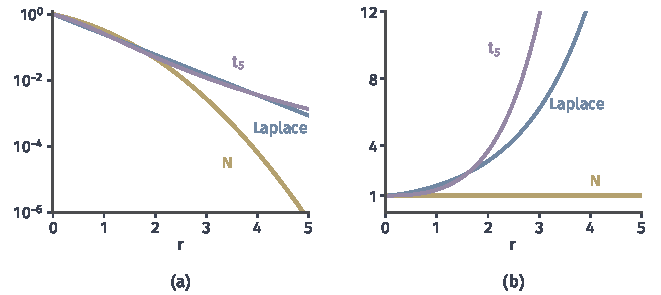
\includegraphics[width=112mm]{figures/07-probability/01-elementary-probability/matplotlib/mvd-model-tails/figure.pdf}
  \caption{均值为$\bm{0}$、协方差为$\bm{I}_2$的三个椭圆模型：高斯（黄）、多元Laplace（蓝）、$\nu=5$的多元t（紫，尺度矩阵$\tfrac35\bm{I}$）。(a)边缘尾概率$\mathbb{P}(\lvert X_1\rvert>r)$，纵轴取对数。(b)联合超越比$\mathbb{P}(\lvert X_1\rvert>r,\lvert X_2\rvert>r)/\mathbb{P}(\lvert X_1\rvert>r)^{2}$，独立时恒为$1$。曲线由对共同尺度的精确密度数值积分得到。}
  \label{fig:mvd-model-tails}
\end{BookInlineFigure}

\paragraph{不相关与独立}
三种实值模型对“不相关能否推出独立”给出不同回答。联合高斯时，零交叉协方差推出独立，定理~\ref{thm:mvd-gaussian-independence}。多元t与多元Laplace中，即使尺度矩阵是对角的，共同尺度也使分量相关于各自的大小，零协方差不推出独立。$(Z,SZ)$说明另一种失效：每个分量都是高斯，但向量不联合高斯，定理同样不适用。

\paragraph{矩与支撑}
矩的存在条件也不同。高斯与Laplace的各阶矩都有限；t分布只有低于$\nu$阶的矩，$\bm{\Sigma}$只在$\nu>2$时通过$\nu/(\nu-2)$与协方差相连。支撑维数则由约束决定：计数与比例都受一条线性约束，住在$d-1$维的格点或单纯形上；退化高斯受$d-r$条线性约束，住在$r$维平面上。凡是有约束的模型，协方差矩阵都奇异，零空间正对应约束方向。

这些比较说明，选择多元模型时要同时核对四件事：取值范围与约束，边缘的尾部，依赖的来源，需要的矩是否存在。只核对均值与协方差，会把本质不同的模型当成可以互换的。
